% ---
% Capitulo de revisão de literatura
% ---


\chapter{Referencial Teórico}\label{referencial_teorico}


\section{O que é DevOps?}

O DevOps é o nivelamento entre as equipes de desenvolvimento e operações no que tange suas interações, mantendo suas funções específicas porém alinhando suas demandas referentes às responsabilidades e processos, visando a disponibilização de um produto ou funcionalidade de forma rápida e confiável.

\begin{figure}[htb] %Figura: Ciclo de vida DevOps
	\centering
	
\includegraphics[width=1\linewidth]{figura1}
	\caption{Ciclo DevOps}
	Fonte: AWS
	\label{fig:figura1}
\end{figure}

As implementações nesse tipo de ambiente fazem uso de ferramentas de automação com o intuito de dinamizar cada vez mais a infraestrutura e torná-la mais programável.

Um dos objetivos mais evidentes do DevOps é a melhoria contínua da comunicação e integração entre desenvolvedores e administradores de infra, transformando o cenário tradicional de isolamento entre essas duas equipes em um ambiente participativo e colaborativo.

Seu objetivo é criar uma cultura de colaboração entre as equipes de desenvolvimento e de operações que permite aumentar o fluxo de trabalho completado - maior frequência de deploys - ao mesmo tempo aumentando a estabilidade e robustez do ambiente de produção.(SATO, 2016).

O DevOps representa muito mais do que simplesmente o uso de ferramentas de automação, é importante observarmos que trata-se de uma quebra de paradigmas e uma mudança na cultura no negócio, uma nova forma de entrega e produção.

Mais do que uma modernização tecnológica, por meio das mais diversas áreas de inovação, é uma oportunidade de evoluir a cultura e os processos da organização. (COSTA, 2017).

\section{Quando é usado?}

A agilidade no processo de deploys citado anteriormente aluz à uma necessidade de amparo para que essa entrega rápida de fato aconteça, e mais do que isso, a demanda por parte dos clientes ou usuários de determinada aplicação, requer cada vez mais velocidade no uso de determinada funcionalidade. Analogamente à revolução industrial do século XX, a mudança na forma de produção de produtos naturalmente está sendo absorvida pela tecnologia, assim, a concepção desse produto deve acompanhar a demanda externa. Nesse sentido, a adaptabilidade e mudança da arquitetura funcional no desenvolvimento de serviços tecnológicos são necessidades relevantes, a cultura DevOps é uma mudança importante nesse ponto.

Segundo uma pesquisa realizada pelo Gartner Group sobre DevOps, em 2015, somente 29\% das organizações pesquisadas tem o modelo atuante em produção. É apresentado ainda que apenas 42\% desses, tem a atuação do DevOps em aplicações móveis.
%Fonte: https://www.itforum365.com.br/tecnologia/como-devops-pode-ser-usado-para-desenvolvimento-de-aplicacoes-moveis/

De acordo com o mesmo grupo o DevOps evoluiria de uma estratégia de nicho para uma estratégia comum sendo empregada por 25\% das organizações do Global 2000\footnote{Forbes Global 2000 é uma classificação anual das 2.000 empresas públicas do mundo pela revista Forbes. O ranking é baseado em quatro critérios: vendas, lucro, ativos e valor de mercado. A lista é publicada desde 2003. Fonte: Wikipédia}.

O uso da cultura DevOps deve ser absorvida na necessidade de versionamento contínuo de determinada aplicação, ou seja, a frequente execução de deploys. Nisso, é importante observarmos que a rápida proliferação de software requer atualizações atuando na mesma medida ágil e a demanda pela competitividade de mercado, visto que a velocidade no atendimento da expectativa dos clientes diferencia a empresa em relação às demais no mercado.


% ############# PESQUISAR E ACRESCENTAR (Ver com o professor)  #######################
%- Levantamento de tarefas com fim na automatização;
%- Definir ferramentas adotadas;
%- Pesquisar sobre práticas ágeis que facilitem o gerenciamento.
% ####################################################################################

\section{Qual o ganho em utilizá-lo?}
A principal vantagem no uso de DevOps é a melhora evidente nos processos e automatização das tarefas, otimizando o tempo e reduzindo os ciclos de desenvolvimento. Por se tratar de uma interação entre as equipes de desenvolvedores e operacionais, dizemos que é um sistema bimodal de trabalho.

O monitoramento de métricas e registro de logs é um aspecto relevante, leva-se em conta que os serviços devem estar disponíveis 24 horas por dias e durante os 07 dias da semana, acarretando numa análise de dados e logs gerados pelo sistema em um nível massivo, portanto, a rotina na observância desses elementos deve ser constante. É possível, inclusive, a criação de alertas que apontem situações e permitam a gerência proativa dos serviços.

Outro benefício fundamental do DevOps é o aumento na comunicação e colaboração que envolve todos os personagens da empresa. É importantíssimo a definição de normas que permitam um maior compartilhamento de informações, ou que permitam a proliferação da comunicação sejam por meio de qualquer que for o método ou tecnologia, desde que agregue valor. Além disso, a diminuição de ruídos na comunicação e conflitos entre as equipes melhora o ambiente e tende a produzir efeitos positivos ao fim do processo.

Podemos ainda elencar ganhos em maior estabilidade e melhor desempenho, e tão importante quanto, a redução considerável de custos de trabalho, visto que a diminuição de tempo de produção e menor esforço afeta diretamente o custo estimado em um projeto.



\section{Microserviços}

Nesse ambiente, um grande sistema pode ser desmembrado em vários sistemas que atuem de forma mais simples e independentes. Dessa forma, é possível gerir melhor as equipes responsáveis e dar mais agilidade ao processo de desenvolvimento.

Esse desacoplamento gera inevitavelmente um número maior de deploys acontecendo simultaneamente. Dessa forma, o DevOps associado a esse cenário potencializa o desempenho de produção e gerência, aplicando a integração e entregas contínuas.

\section{Infraestrutura como Código}

\section{Principais Ferramentas e Recursos Tecnológicos Disponíveis}
Apesar do conceito DevOps ser recente, a gama de ferramentas que contribuem para implantação dessa cultura já se mostram bastante diversificadas. Dentre as mais comuns podemos apresentar:

\subsection{Atlas}
É uma ferramenta disponibilizada pela Hashicorp, que tem a função de unificar projetos open source para o manejo de aplicações finalizadas no desenvolvimento para a produção em qualquer que seja a infraestrutura.
As etapas do Atlas seguem cinco passos (Figura 2), isso independe da tecnologia utilizada, sejam máquinas virtuais ou contêineres, as etapas se mantêm as mesmas.

\begin{figure}[htb]
	\centering
	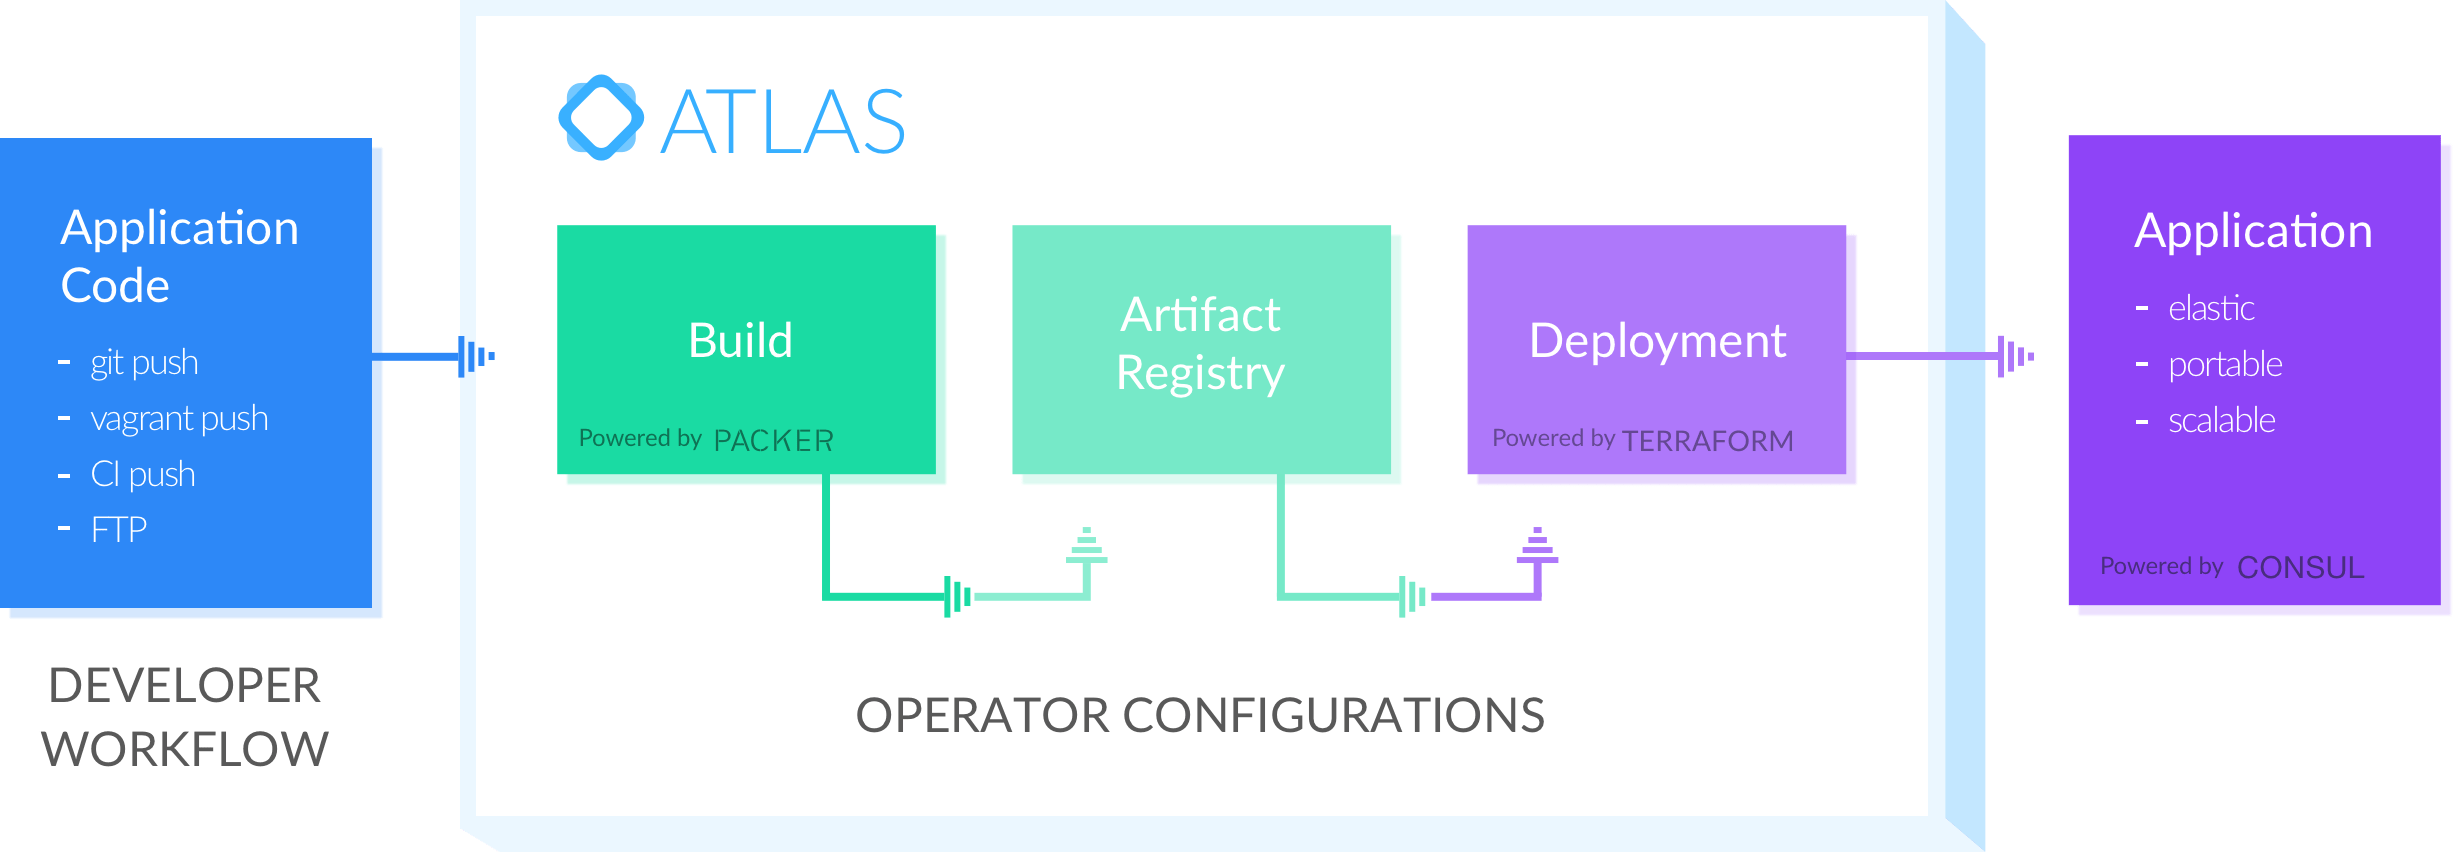
\includegraphics[width=0.8\linewidth]{etatasAtlas}
	\caption{Etapas do Atlas}
	Fonte: Hashicorp
	\label{fig:etatasAtlas}
\end{figure}

O Atlas não é um software de caixa preta, ou seja, é possível acesso a serviços que contribuem para tanto, como Vagrant (gerencia ambientes de desenvolvimento), Packer (construção de artefatos), Terraform (implantação de Infraestrutura) e Consul (monitora os serviços em tempo real).

\subsection{Chef}
É um framework destinado à automatização para sistemas e infraestrutura em nuvem. O Chef\footnote{Disponível em https://www.chef.io} constrói, entrega e administra fazendo uso de scripts replicáveis.

O Chef tira a carga dos administradores de sistemas que focam no gerenciamento projetado para servidores autônomos, ele permite executar cetenas de instâncias de servidor em um tempo imensamente maior se comparado ao uso comum em deploys.

Para gerenciar esse tipo de configuração, o Chef, transforma a infraestrutura em código, deixando o processo mais flexível, legível pelos analistas e testável, possibilitando assim a gerência de recursos tanto localmente quanto na nuvem

Em sua topologia o Chef tem três principais componentes: o Servidor Chef, as Estações e o Nós.

O maior atrativo dessa ferramenta é o uso de "cookbooks" ou receitas, são ditas configurações plugáveis, que envolvem todas as instalações e parâmetros necessários para atender determinada aplicação no servidor ou máquina. Assim como as receitas convencionais definem uma estrutura sequencial que deve ser seguida a fim de tornar o produto final reflexo de uma ideia original, o Chef mantém um conceito semelhante a isso, onde define-se um estado desejado do sistema, desenvolvendo um código de configuração, então o ele processa esse código, une ao processo os dados do nó em questão e garante que o estado concebido seja correspondente ao estado do sistema. 

O Chef pode ser executado em várias plataformas, como Windows, distribuições Linux, FreeBSD, Solaris, AIX, Cisco IO e Nexus. E ainda suporta plataformas em nuvem,como Amazon Web Services $($AWS$)$, Google Cloud Platform, OpenStack, IBM Bluemix, HPE Cloud, Microsoft Azure e VMware vRealize.

\subsection{Docker}

O Docker\footnote{Disponível em https://www.docker.com/}. é uma plataforma de automação que implanta as aplicações em espaços isolados chamados de \textit{containers}, possibilitando as executarem as aplicações de forma mais ágil. O objetvo é criar múltiplos ambientes dentro de um mesmo servidor, acessíveis externamente.

O Docker é uma plataforma Open Source, que não pode ser confundido com um ambiente tradicional de virtualização. No Docker fazemos uso de recurso isolados que utilizam bibliotecas do kernel em comum, isso porque é presente nessa ferramenta o Linux Containers (LXC).

Com ele é possível empacotar a aplicação ou um ambiente em um contêiner e movê-lo para qualquer outro host que possua o Docker instalado, tornando assim uma ferramenta portável. A grande vantagem disso é que não há necessidade de reconfigurar todo o ambiente novamente, visto que todo ele é movido, reduzindo acentuadamente o tempo de deploy de uma infraestrutura.

Essa plataforma não pode ser confundida com um ambiente virtualizado, visto que em cenários que utilizam máquinas virtuais há a presença de uma camada intermediária de sistema operacional entre o host e as aplicações, no Docker essa é desnecessária pois ele não utiliza kernel, tornando independente quanto a nível de disco, memória e processamento.

\begin{figure} [htb]
\centering
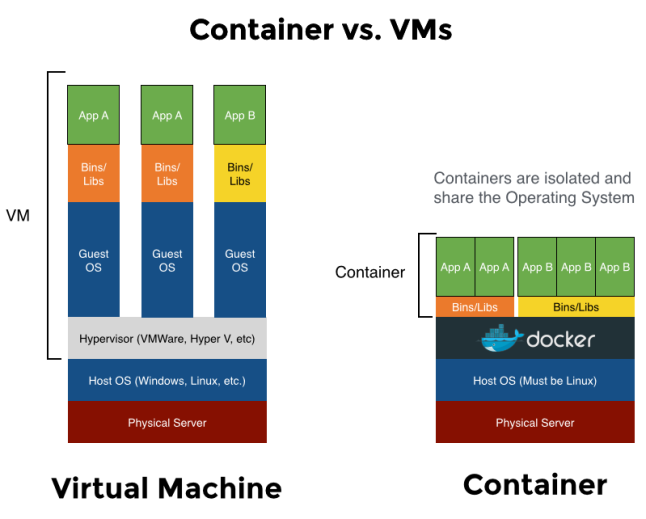
\includegraphics[width=0.7\linewidth]{imagens/dockerXvm}
\caption{Comparativo Docker x Máquinas Virtuais}
\label{fig:dockerXvm}
\end{figure}


A infraestrutura no Docker também é replicável, é possível criar imagens predefinidas e disponibilizá-las em ambientes de desenvolvimento, teste, homologação e produção para aplicações.

\subsection{Puppet}
É uma ferramenta de código livre para gestão de configurações. A ideia central do Puppet\footnote{Disponível em https://www.puppet.com/} é a administração de diversas máquinas físicas ou virtuais, onde a configuração é centralizada em um único nó e então distribuídas por diversos nós na rede, assim, gerenciando configurações, automatizando instalação de pacotes e facilitando o estabelecimento de normas e auditoria.

A ferramenta está disponível em duas versões: Puppet Enterprise $($com suporte pago$)$, e a Open Source Puppet $($código aberto$)$. É uma ferramenta bem utilizada pela comunidade e por isso existem muitos módulos desenvolvidos, empresas como McAfee e Nasa fazem uso dela.

O Puppet utiliza SSH para a conexão aos hosts, esse é um ponto positivo se olharmos pela ótica que em alguns cenários não é possível a instalação de agentes ou em situações onde o agente consome uma fatia considerável de memória e cpu.



\begin{figure} [htb]
	\centering
	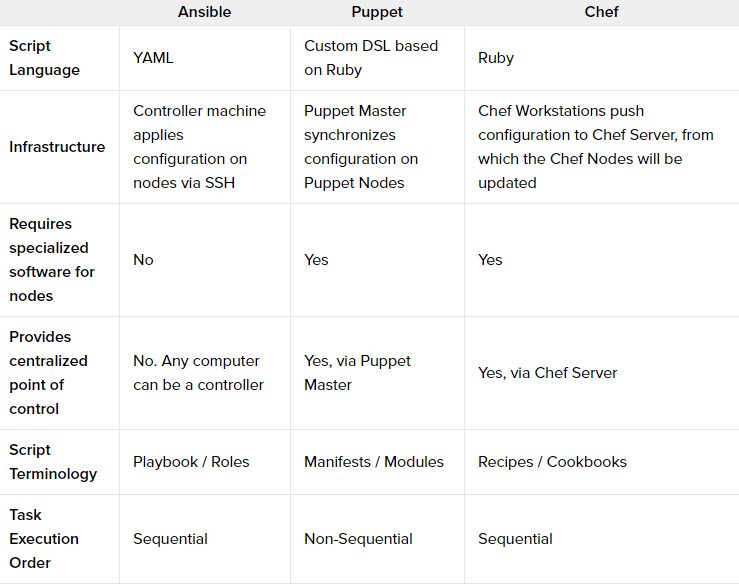
\includegraphics[width=0.7\linewidth]{puppet}
	\caption{Comparativo entre Ferramentas de Gerenciamento de Configurações}
	Fonte: Digital Ocean
	\label{fig:puppet}
\end{figure}


\subsection{Ansible}

O Ansible\footnote{Disponível em https://www.ansible.com} oferece duas versões, o Ansible Core, que é a versão gratuita e de código aberto, e o Ansible Tower, versão comercial.

O Ansible orquestra os nós implementando módulos para nós sobre SSH. Os módulos são distribuídos nos nós temporariamente que realizam a comunicação com a máquina de controle (assim com em ferramentas concorrentes) por meio de um protocolo JSON.
O diferencial do Ansible em relação as demais ferramentas que se propõe ao mesmo objetivo, é que ele atua com uma arquitetura cliente-servidor, sem agente,  isso que dizer que os nós não são necessários para a instalação dos daemons para comunicação com a máquina controle. Isso resulta em diminuição de carga na rede. 

Nessa ferramenta ainda encontramos o uso de um arquivo de inventário, denominado "hosts", que definem quais nós serão gerenciados, que é simplesmente um arquivo de texto que lista os nós individualmente ou agrupados ou até um arquivo executável que constrói um inventário de hosts.

Na forma tradicional de trabalho o Ansible faz o upload do código que deve ser executado nas estações clientes, é então executado, retorna o resultado da execução e após isso é removido dos clientes.

Quando usamos a ótica DevOps esse tipo de fluxo é modificado, fazendo uso do protocolo NETCONF $($RFC 6241$)$, onde é possivel o envio de comandos aos componentes e receber o retorno da aplicação.


\subsection{GITHUB}
É um dos serviços web mais difundidos. Com essa ferramenta é possível hospedar projetos e aplicações, trabalhando com controle de versionamento.

O Github\footnote{Disponível em https://www.github.com} funciona por meio de repositórios, que funcionam como pastas e dentro destas outras pastas que comportam os arquivos de diversas extensões e linguagens. Ainda oferece a possibilidade de contribuir com um determinado para o desenvolvimento de determinado projeto. Além, e permitir o acesso múltiplo por diversos desenvolvedores de um mesma empresa, permitindo que vários programadores trabalhem simultaneamente em uma mesma aplicação ou arquivo.

\begin{figure} [htb]
	\centering
	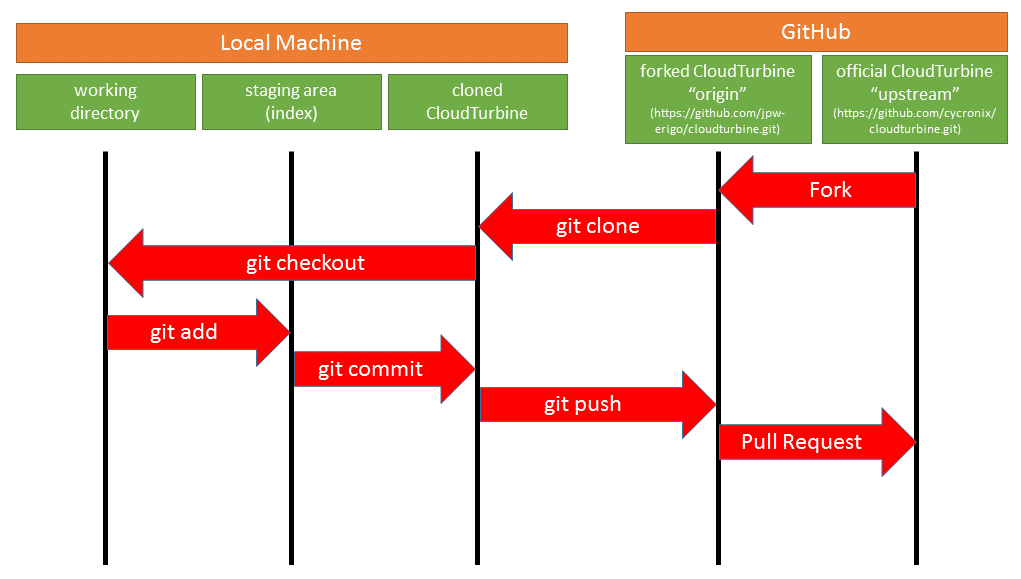
\includegraphics[width=0.7\linewidth]{git}
	\caption{Fluxo commit e request}
	Fonte: Cloud Turbine
	\label{fig:git}
\end{figure}

\subsection{Jenkins}
Essa ferramenta multiplataforma e funciona como um servidor destinado a integração contínua que automatiza a execução de tarefas, possui código aberto e permite ao usuário total liberdade em sua operação.

O Jenkins\footnote{Disponível em https://www.jenkins.io} pode ser integrado ao Git, SVN, CVS, Maven, entre outros. É importante ressaltar que um ponto forte do Jenkins é a difusão entre a comunidade.

Um recurso interessante é o uso de Forks $($recurso do GitHub$)$, que permitem a criação de cópias de um determinado projeto e trabalha nesse sem a preocupação de afetar em algum ponto a aplicação original.

É possivel ainda, adicionar testes de desempenho e balanceamento na integração contínua, permitindo a análise de risco e a reduzir eventuais quedas de performance no momento em que um novo recurso é adicionado ou a correção de um erro presente.

% ############ ADICIONAR DIAGRAMA (VER COM O PROFESSOR)




